
\section{\popTwoII}

\TODO{kjghcvgkh}

\section{things to do bla}
	
\TODO{more data, depths, surface intensified, upper layer}

\TODO{ Further study in refining this structure is expected, and the refined structure can serve as a benchmark for numerical models where mesoscale eddies are explicitly resolved. In addition, the generation mechanism for this universal structure remains unknown; thus, exploring such mechanism may bring new excitement to eddy research.} -Zhang2013 }

\TODO{3d structure still mystery}

\TODO{H/f contours}

\TODO{tracers AC/C diff}

%%....................................F.I.G.U.R.E.............................................
\begin{figure}
	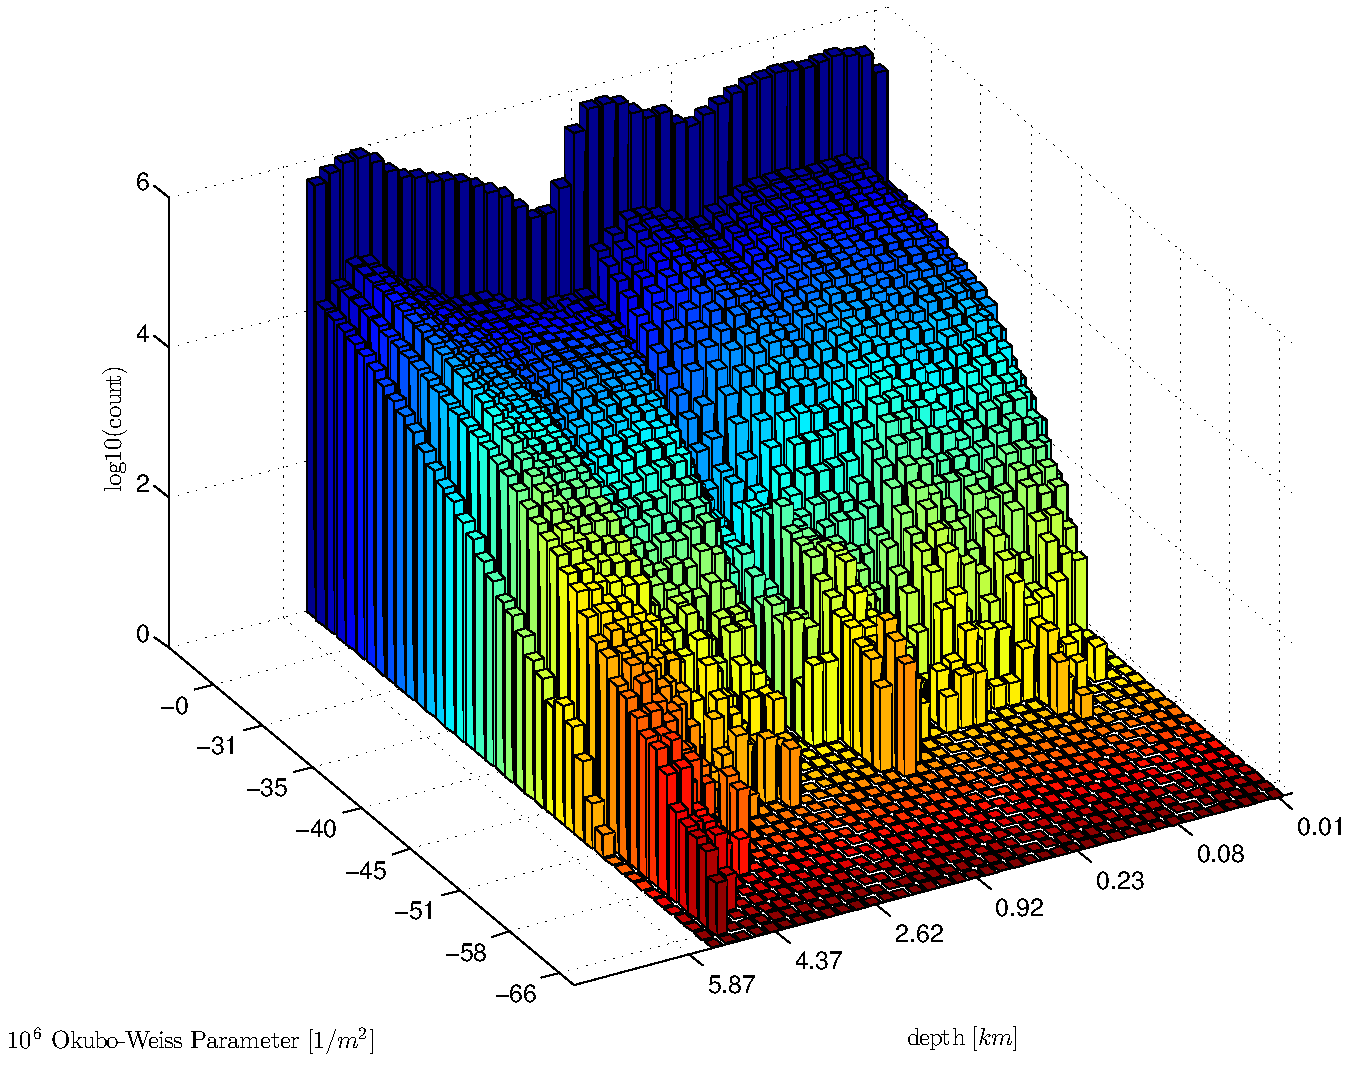
\includegraphics[]{OW_count-OW-depth}
	\caption{Histogram of global $\okubo$ as a function of depth calculated from \POP~$\vec{u}$-data. The idea was to find the surface $z_{ow}(y,x)$ of minimum $\okubo(z,y,x)$ and then use that depth as the depth to take the mean current from (see \cref{subsection:netU}). The maximum tends to be at the ocean floor which led to the conjecture that the numerical implementation of $\okubo$ might have been erronuos. Further applcation was hence abandoned.  }
	\label{fig:OW_count-OW-depth}
\end{figure}
%%....................................F.I.G.U.R.E.............................................


\begin{figure}
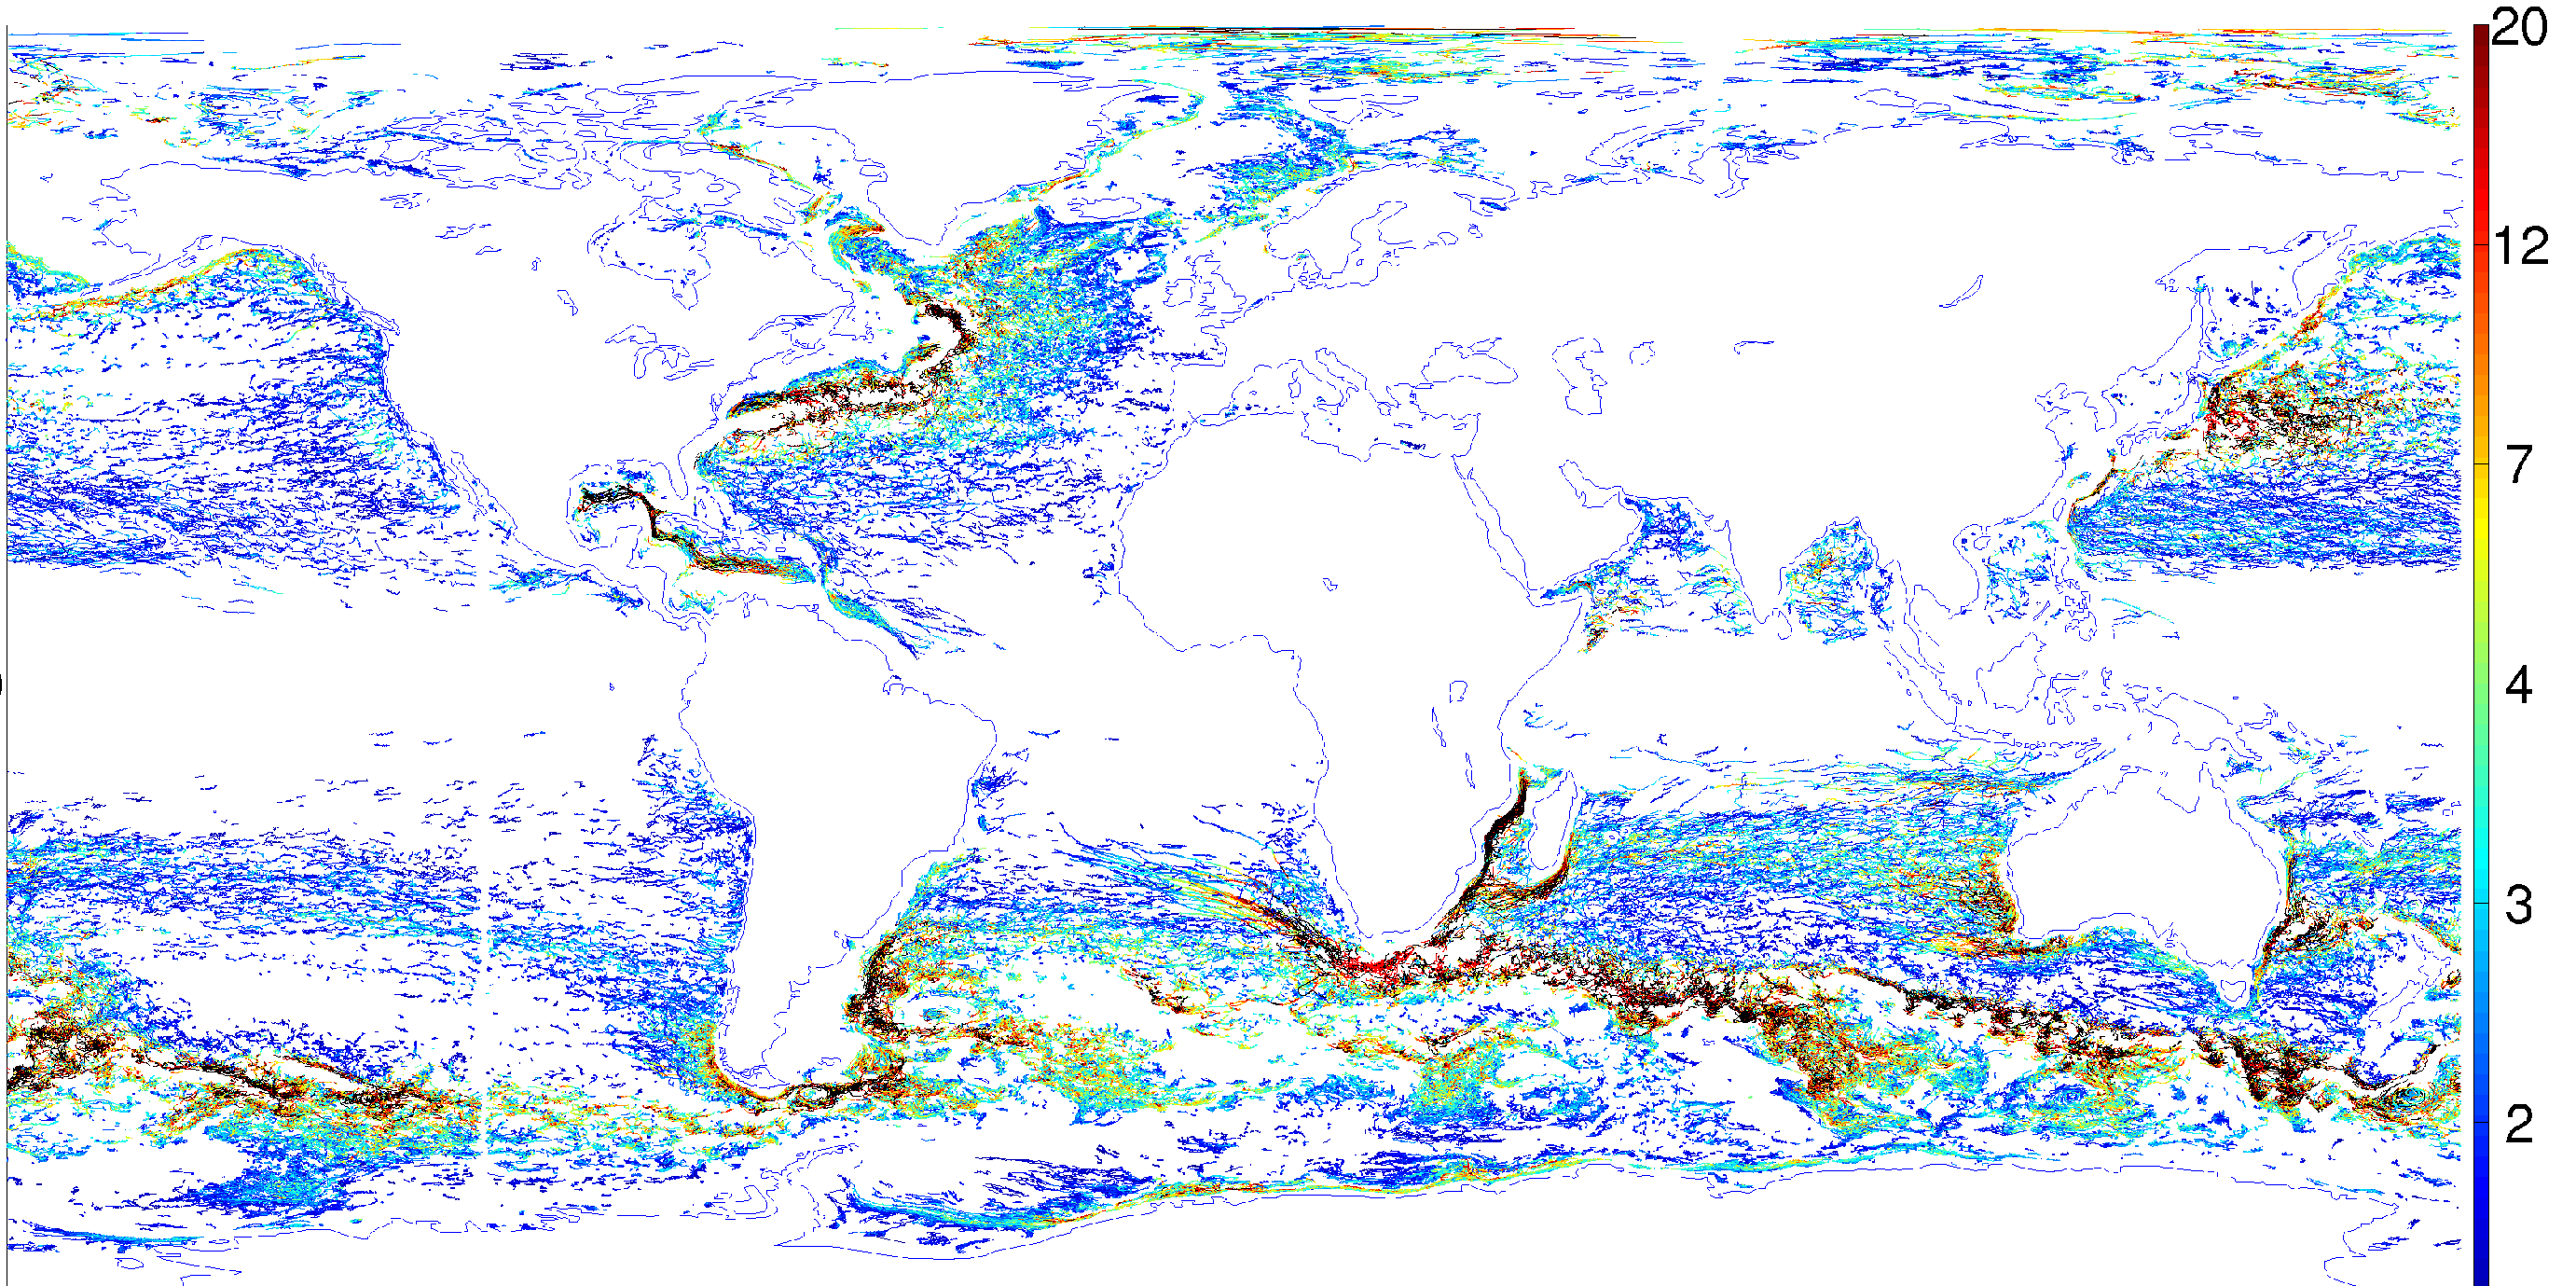
\includegraphics[]{TrackPeakampto_ellipseAntiCycsCrpd}
\caption{Amplitude $\Unit{\si{\cm}}$ (w.r. to contour). Tracks are from very early \POP~test-runs.}
\label{fig:TrackPeakampto_ellipseAntiCycsCrpd}
\end{figure}
